
% Results
In this chapter we present the results of the gridsearch we conducted in the process of parameter optimization. Using accuracy as a measure for the classification quality we evaluated the effects of feature and data selection on the generalization ability of our machine learning algorithms.\\
Classification accuracy has been calculated from classifier validation (i.e. using the trained estimator to make predictions on the reserved test data).\\

The results of the validation process are shown in the graphs below. We used a series of bar plots to visualize the accuracies we achieved with each classifier for each data set based on the used feature set. Plots are distinguished by feature selection and crossvalidation. Data sets, on the x-axis, are plotted against accuracy, on the y-axis. The bars are color coded to indicate machine learning algorithms.\\

% original feature set CV 3
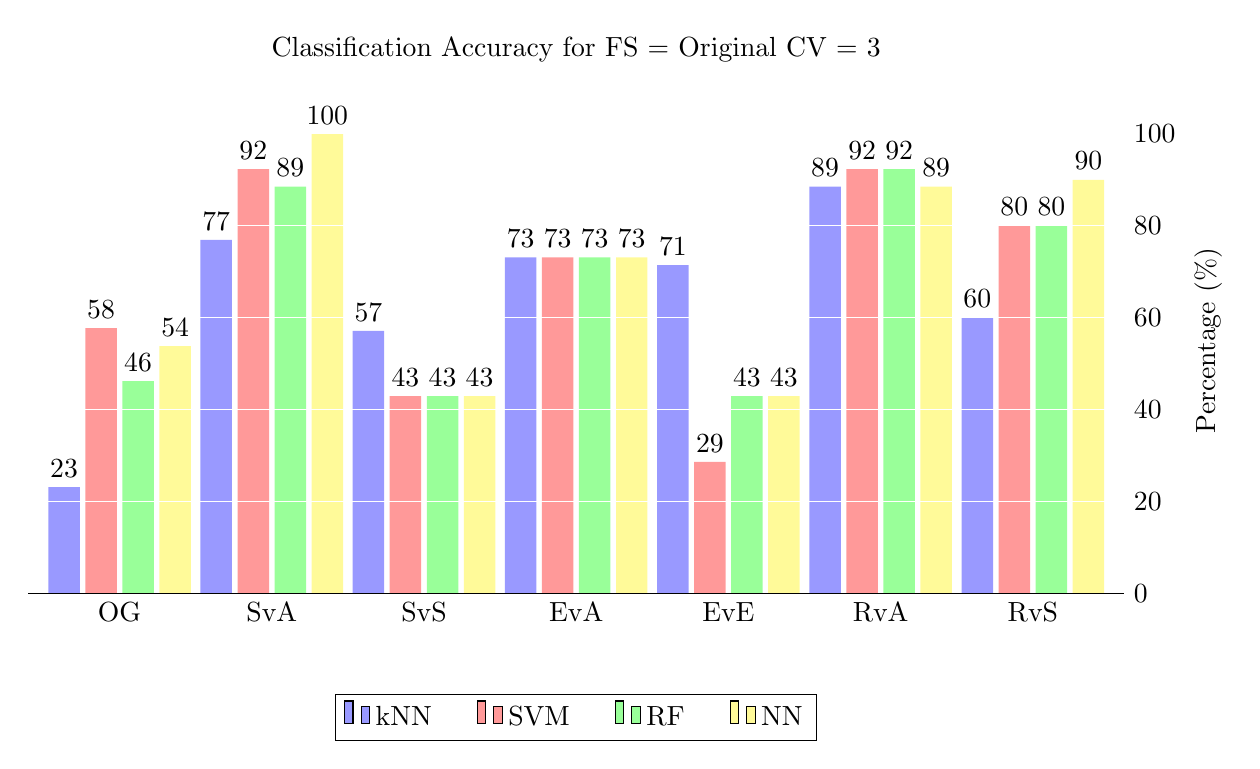
\begin{tikzpicture}
  \centering
  \begin{axis}[
        ybar, axis on top,
        title={Classification Accuracy for FS = Original CV = 3},
        height=8cm, width=15.5cm,
        bar width=0.4cm,
        ymajorgrids, tick align=inside,
        major grid style={draw=white},
        enlarge y limits={value=.1,upper},
        ymin=0, ymax=100,
        axis x line*=bottom,
        axis y line*=right,
        y axis line style={opacity=0},
        tickwidth=0pt,
        enlarge x limits=true,
        legend style={
            at={(0.5,-0.2)},
            anchor=north,
            legend columns=-1,
            /tikz/every even column/.append style={column sep=0.5cm}
        },
        ylabel={Percentage (\%)},
        symbolic x coords={
           OG, 
           SvA, 
           SvS, 
           EvA, 
           EvE, 
           RvA, 
           RvS},
       xtick=data,
       nodes near coords={
        \pgfmathprintnumber[precision=0]{\pgfplotspointmeta}
       }
    ]
    % kNN
    \addplot [draw=none, fill=blue!40] coordinates {
      (OG, 23.1)
      (SvA, 76.9) 
      (SvS, 57.1)
      (EvA, 73.1) 
      (EvE, 71.4) 
      (RvA, 88.5)
      (RvS, 60.0) };
   % SVM
   \addplot [draw=none,fill=red!40] coordinates {
      (OG, 57.7)
      (SvA, 92.3) 
      (SvS, 42.9)
      (EvA, 73.1) 
      (EvE, 28.6) 
      (RvA, 92.3)
      (RvS, 80.0) };
   % RF
   \addplot [draw=none, fill=green!40] coordinates {
      (OG, 46.2)
      (SvA, 88.5) 
      (SvS, 42.9)
      (EvA, 73.1) 
      (EvE, 42.9) 
      (RvA, 92.3)
      (RvS, 80.0) };
   % NN
   \addplot [draw=none, fill=yellow!40] coordinates {
      (OG, 53.8)
      (SvA, 100) 
      (SvS, 42.9)
      (EvA, 73.1) 
      (EvE, 42.9) 
      (RvA, 88.5)
      (RvS, 90.0) };

    \legend{kNN,SVM,RF,NN}
  \end{axis}
\end{tikzpicture}

% original feature set CV 5
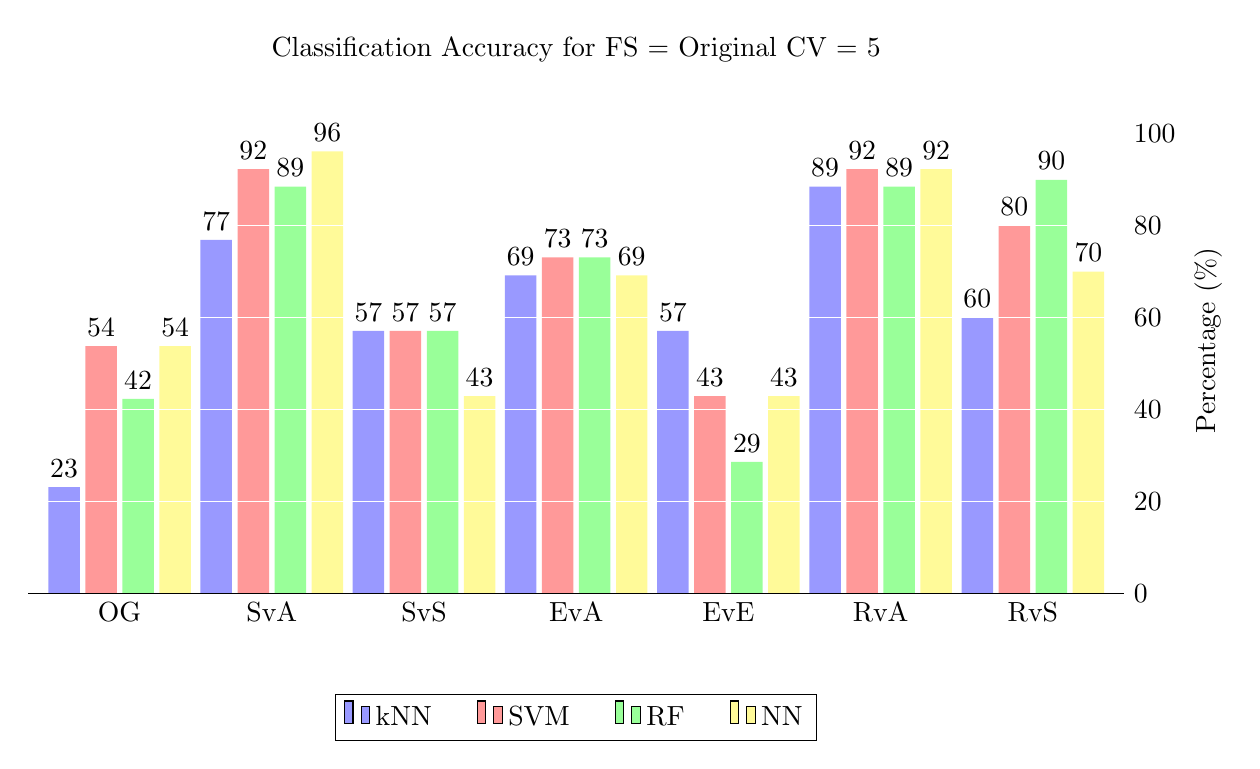
\begin{tikzpicture}
  \centering
  \begin{axis}[
        ybar, axis on top,
        title={Classification Accuracy for FS = Original CV = 5},
        height=8cm, width=15.5cm,
        bar width=0.4cm,
        ymajorgrids, tick align=inside,
        major grid style={draw=white},
        enlarge y limits={value=.1,upper},
        ymin=0, ymax=100,
        axis x line*=bottom,
        axis y line*=right,
        y axis line style={opacity=0},
        tickwidth=0pt,
        enlarge x limits=true,
        legend style={
            at={(0.5,-0.2)},
            anchor=north,
            legend columns=-1,
            /tikz/every even column/.append style={column sep=0.5cm}
        },
        ylabel={Percentage (\%)},
        symbolic x coords={
           OG, 
           SvA, 
           SvS, 
           EvA, 
           EvE, 
           RvA, 
           RvS},
       xtick=data,
       nodes near coords={
        \pgfmathprintnumber[precision=0]{\pgfplotspointmeta}
       }
    ]
    % kNN
    \addplot [draw=none, fill=blue!40] coordinates {
      (OG, 23.1)
      (SvA, 76.9) 
      (SvS, 57.1)
      (EvA, 69.2) 
      (EvE, 57.1) 
      (RvA, 88.5)
      (RvS, 60.0) };
   % SVM
   \addplot [draw=none,fill=red!40] coordinates {
      (OG, 53.8)
      (SvA, 92.3) 
      (SvS, 57.1)
      (EvA, 73.1) 
      (EvE, 42.9) 
      (RvA, 92.3)
      (RvS, 80.0) };
   % RF
   \addplot [draw=none, fill=green!40] coordinates {
      (OG, 42.3)
      (SvA, 88.5) 
      (SvS, 57.1)
      (EvA, 73.1) 
      (EvE, 28.6) 
      (RvA, 88.5)
      (RvS, 90.0) };
   % NN
   \addplot [draw=none, fill=yellow!40] coordinates {
      (OG, 53.8)
      (SvA, 96.2) 
      (SvS, 42.9)
      (EvA, 69.2) 
      (EvE, 42.9) 
      (RvA, 92.3)
      (RvS, 70.0) };

    \legend{kNN,SVM,RF,NN}
  \end{axis}
\end{tikzpicture}

% reduced (time) feature set CV 3
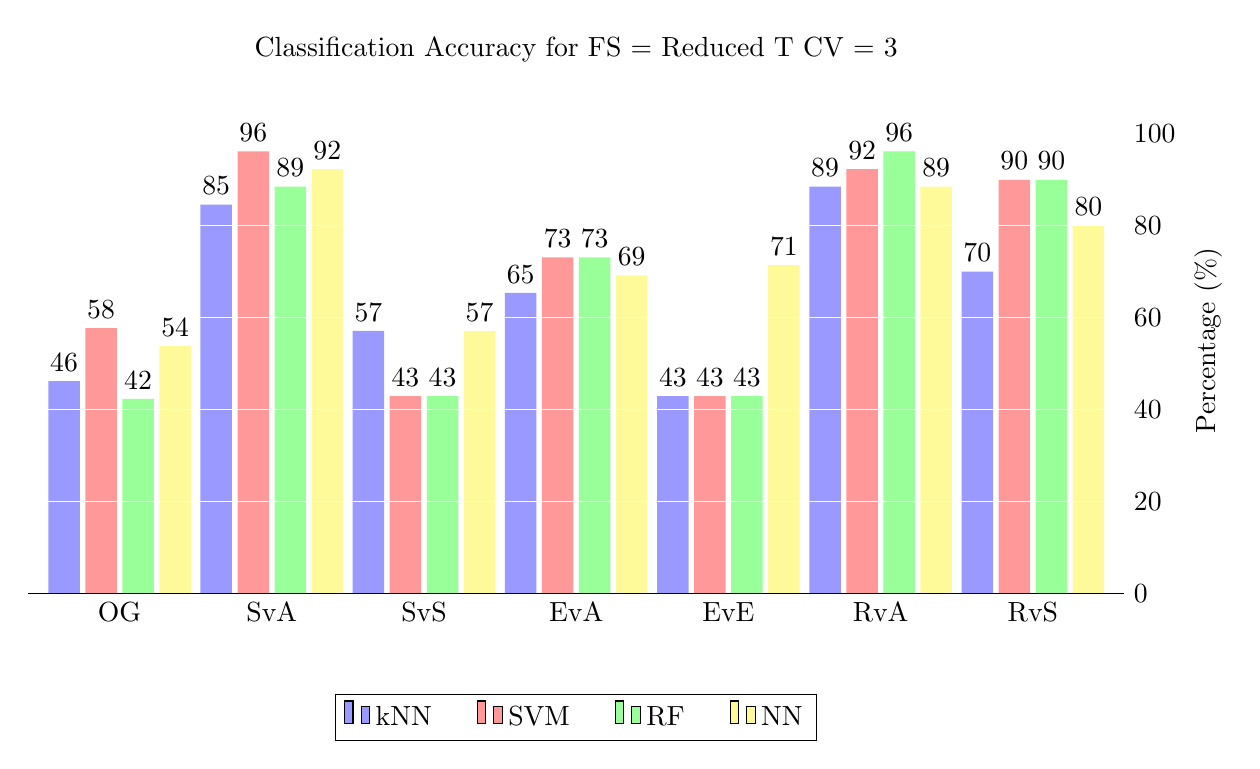
\begin{tikzpicture}
  \centering
  \begin{axis}[
        ybar, axis on top,
        title={Classification Accuracy for FS = Reduced T CV = 3},
        height=8cm, width=15.5cm,
        bar width=0.4cm,
        ymajorgrids, tick align=inside,
        major grid style={draw=white},
        enlarge y limits={value=.1,upper},
        ymin=0, ymax=100,
        axis x line*=bottom,
        axis y line*=right,
        y axis line style={opacity=0},
        tickwidth=0pt,
        enlarge x limits=true,
        legend style={
            at={(0.5,-0.2)},
            anchor=north,
            legend columns=-1,
            /tikz/every even column/.append style={column sep=0.5cm}
        },
        ylabel={Percentage (\%)},
        symbolic x coords={
           OG, 
           SvA, 
           SvS, 
           EvA, 
           EvE, 
           RvA, 
           RvS},
       xtick=data,
       nodes near coords={
        \pgfmathprintnumber[precision=0]{\pgfplotspointmeta}
       }
    ]
    % kNN
    \addplot [draw=none, fill=blue!40] coordinates {
      (OG, 46.2)
      (SvA, 84.6) 
      (SvS, 57.1)
      (EvA, 65.4) 
      (EvE, 42.9) 
      (RvA, 88.5)
      (RvS, 70.0) };
   % SVM
   \addplot [draw=none,fill=red!40] coordinates {
      (OG, 57.7)
      (SvA, 96.2) 
      (SvS, 42.9)
      (EvA, 73.1) 
      (EvE, 42.9) 
      (RvA, 92.3)
      (RvS, 90.0) };
   % RF
   \addplot [draw=none, fill=green!40] coordinates {
      (OG, 42.3)
      (SvA, 88.5) 
      (SvS, 42.9)
      (EvA, 73.1) 
      (EvE, 42.9) 
      (RvA, 96.2)
      (RvS, 90.0) };
   % NN
   \addplot [draw=none, fill=yellow!40] coordinates {
      (OG, 53.8)
      (SvA, 92.3) 
      (SvS, 57.1)
      (EvA, 69.2) 
      (EvE, 71.4) 
      (RvA, 88.5)
      (RvS, 80.0) };

    \legend{kNN,SVM,RF,NN}
  \end{axis}
\end{tikzpicture}

% reduced (time) feature set CV 5
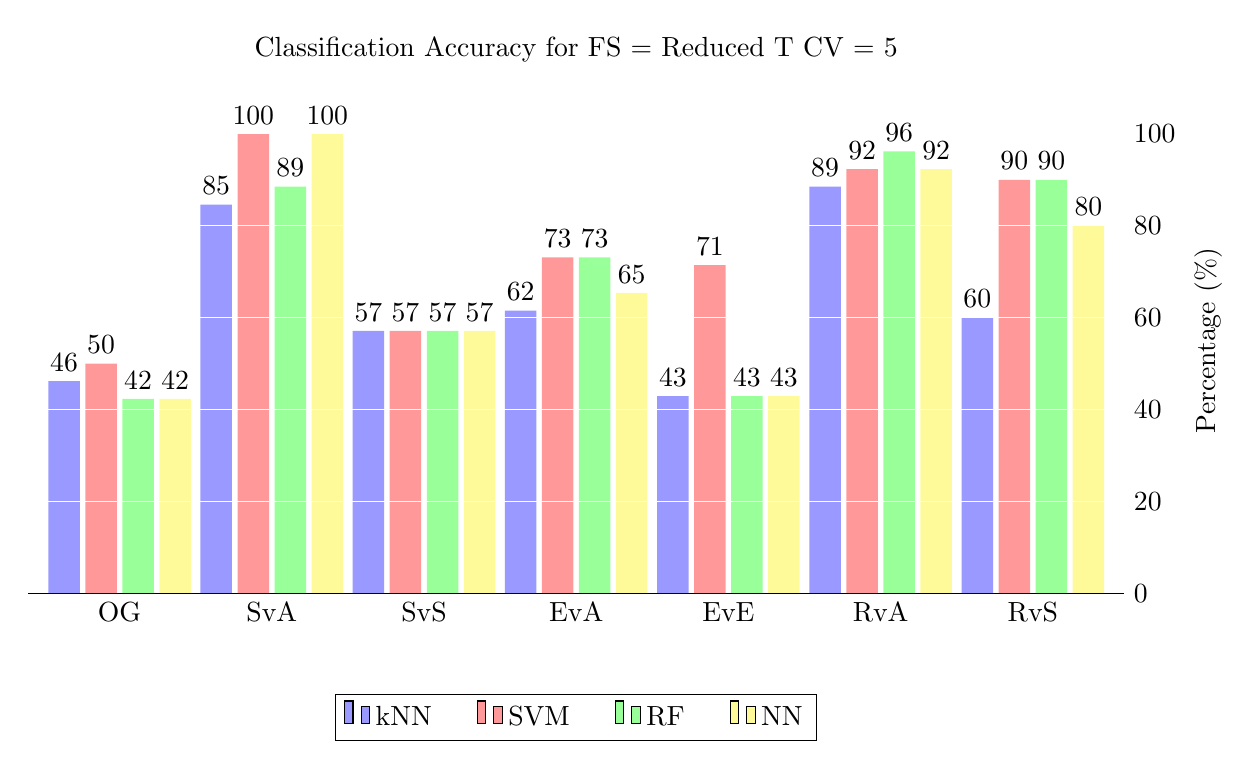
\begin{tikzpicture}
  \centering
  \begin{axis}[
        ybar, axis on top,
        title={Classification Accuracy for FS = Reduced T CV = 5},
        height=8cm, width=15.5cm,
        bar width=0.4cm,
        ymajorgrids, tick align=inside,
        major grid style={draw=white},
        enlarge y limits={value=.1,upper},
        ymin=0, ymax=100,
        axis x line*=bottom,
        axis y line*=right,
        y axis line style={opacity=0},
        tickwidth=0pt,
        enlarge x limits=true,
        legend style={
            at={(0.5,-0.2)},
            anchor=north,
            legend columns=-1,
            /tikz/every even column/.append style={column sep=0.5cm}
        },
        ylabel={Percentage (\%)},
        symbolic x coords={
           OG, 
           SvA, 
           SvS, 
           EvA, 
           EvE, 
           RvA, 
           RvS},
       xtick=data,
       nodes near coords={
        \pgfmathprintnumber[precision=0]{\pgfplotspointmeta}
       }
    ]
    % kNN
    \addplot [draw=none, fill=blue!40] coordinates {
      (OG, 46.2)
      (SvA, 84.6) 
      (SvS, 57.1)
      (EvA, 61.5) 
      (EvE, 42.9) 
      (RvA, 88.5)
      (RvS, 60.0) };
   % SVM
   \addplot [draw=none,fill=red!40] coordinates {
      (OG, 50.0)
      (SvA, 100.0) 
      (SvS, 57.1)
      (EvA, 73.1) 
      (EvE, 71.4) 
      (RvA, 92.3)
      (RvS, 90.0) };
   % RF
   \addplot [draw=none, fill=green!40] coordinates {
      (OG, 42.3)
      (SvA, 88.5) 
      (SvS, 57.1)
      (EvA, 73.1) 
      (EvE, 42.9) 
      (RvA, 96.2)
      (RvS, 90.0) };
   % NN
   \addplot [draw=none, fill=yellow!40] coordinates {
      (OG, 42.3)
      (SvA, 100.0) 
      (SvS, 57.1)
      (EvA, 65.4) 
      (EvE, 42.9) 
      (RvA, 92.3)
      (RvS, 80.0) };

    \legend{kNN,SVM,RF,NN}
  \end{axis}
\end{tikzpicture}

% reduced (freq) feature set CV 3
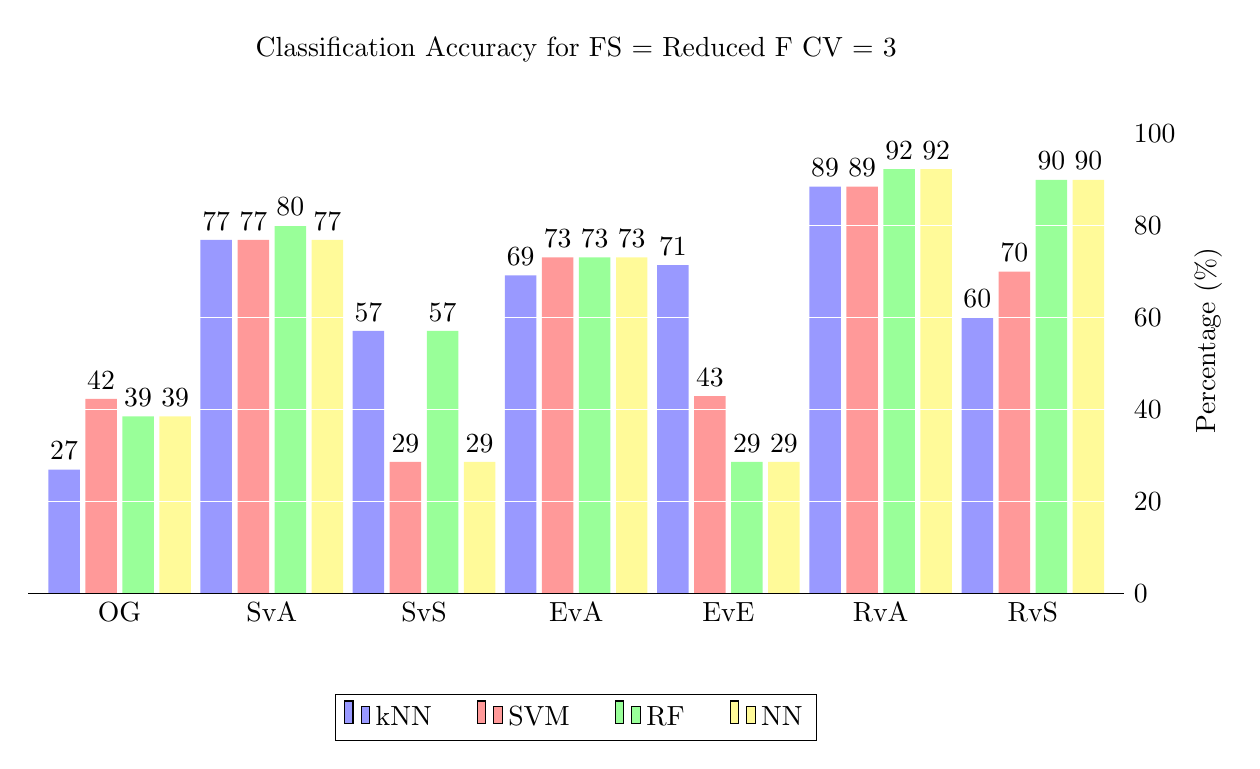
\begin{tikzpicture}
  \centering
  \begin{axis}[
        ybar, axis on top,
        title={Classification Accuracy for FS = Reduced F CV = 3},
        height=8cm, width=15.5cm,
        bar width=0.4cm,
        ymajorgrids, tick align=inside,
        major grid style={draw=white},
        enlarge y limits={value=.1,upper},
        ymin=0, ymax=100,
        axis x line*=bottom,
        axis y line*=right,
        y axis line style={opacity=0},
        tickwidth=0pt,
        enlarge x limits=true,
        legend style={
            at={(0.5,-0.2)},
            anchor=north,
            legend columns=-1,
            /tikz/every even column/.append style={column sep=0.5cm}
        },
        ylabel={Percentage (\%)},
        symbolic x coords={
           OG, 
           SvA, 
           SvS, 
           EvA, 
           EvE, 
           RvA, 
           RvS},
       xtick=data,
       nodes near coords={
        \pgfmathprintnumber[precision=0]{\pgfplotspointmeta}
       }
    ]
    % kNN
    \addplot [draw=none, fill=blue!40] coordinates {
      (OG, 26.9)
      (SvA, 76.9) 
      (SvS, 57.1)
      (EvA, 69.2) 
      (EvE, 71.4) 
      (RvA, 88.5)
      (RvS, 60.0) };
   % SVM
   \addplot [draw=none,fill=red!40] coordinates {
      (OG, 42.3)
      (SvA, 76.9) 
      (SvS, 28.6)
      (EvA, 73.1) 
      (EvE, 42.9) 
      (RvA, 88.5)
      (RvS, 70.0) };
   % RF
   \addplot [draw=none, fill=green!40] coordinates {
      (OG, 38.5)
      (SvA, 80.0) 
      (SvS, 57.1)
      (EvA, 73.1) 
      (EvE, 28.6) 
      (RvA, 92.3)
      (RvS, 90.0) };
   % NN
   \addplot [draw=none, fill=yellow!40] coordinates {
      (OG, 38.5)
      (SvA, 76.9) 
      (SvS, 28.6)
      (EvA, 73.1) 
      (EvE, 28.6) 
      (RvA, 92.3)
      (RvS, 90.0) };

    \legend{kNN,SVM,RF,NN}
  \end{axis}
\end{tikzpicture}

% reduced (freq) feature set CV 5
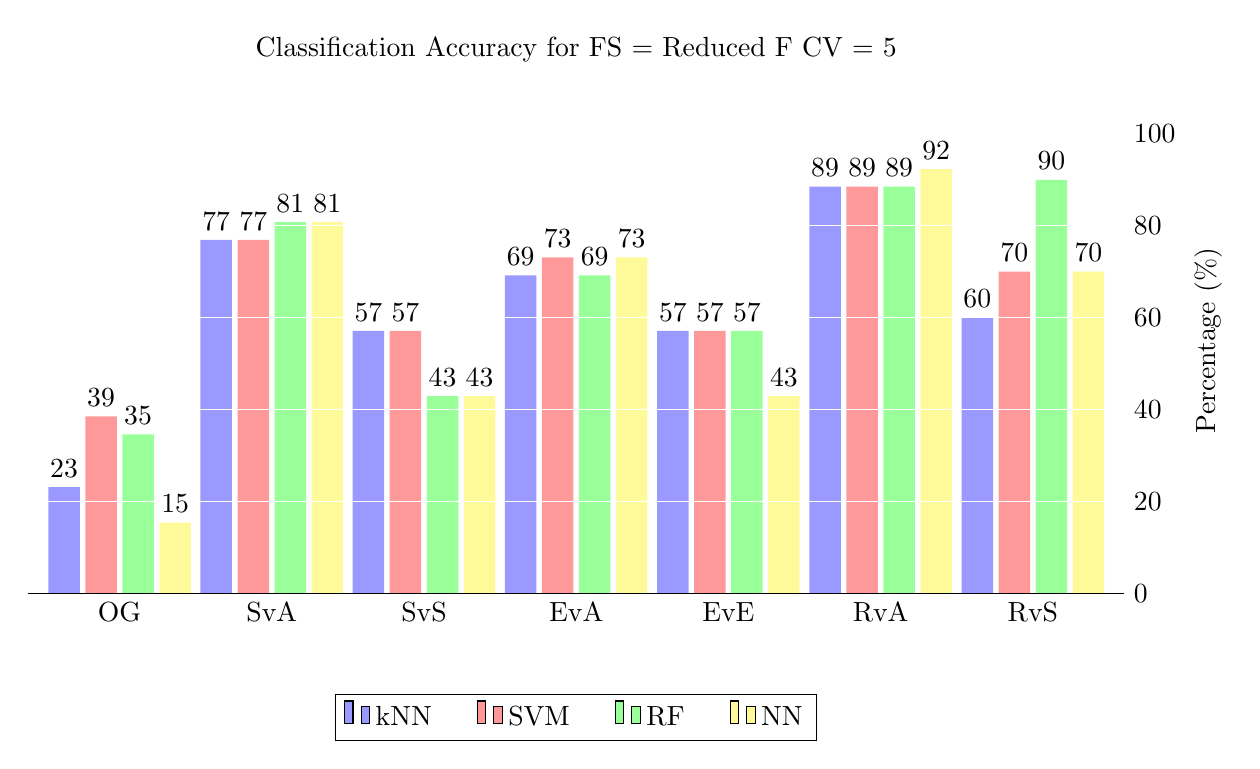
\begin{tikzpicture}
  \centering
  \begin{axis}[
        ybar, axis on top,
        title={Classification Accuracy for FS = Reduced F CV = 5},
        height=8cm, width=15.5cm,
        bar width=0.4cm,
        ymajorgrids, tick align=inside,
        major grid style={draw=white},
        enlarge y limits={value=.1,upper},
        ymin=0, ymax=100,
        axis x line*=bottom,
        axis y line*=right,
        y axis line style={opacity=0},
        tickwidth=0pt,
        enlarge x limits=true,
        legend style={
            at={(0.5,-0.2)},
            anchor=north,
            legend columns=-1,
            /tikz/every even column/.append style={column sep=0.5cm}
        },
        ylabel={Percentage (\%)},
        symbolic x coords={
           OG, 
           SvA, 
           SvS, 
           EvA, 
           EvE, 
           RvA, 
           RvS},
       xtick=data,
       nodes near coords={
        \pgfmathprintnumber[precision=0]{\pgfplotspointmeta}
       }
    ]
    % kNN
    \addplot [draw=none, fill=blue!40] coordinates {
      (OG, 23.1)
      (SvA, 76.9) 
      (SvS, 57.1)
      (EvA, 69.2) 
      (EvE, 57.1) 
      (RvA, 88.5)
      (RvS, 60.0) };
   % SVM
   \addplot [draw=none,fill=red!40] coordinates {
      (OG, 38.5)
      (SvA, 76.9) 
      (SvS, 57.1)
      (EvA, 73.1) 
      (EvE, 57.1) 
      (RvA, 88.5)
      (RvS, 70.0) };
   % RF
   \addplot [draw=none, fill=green!40] coordinates {
      (OG, 34.6)
      (SvA, 80.8) 
      (SvS, 42.9)
      (EvA, 69.2) 
      (EvE, 57.1) 
      (RvA, 88.5)
      (RvS, 90.0) };
   % NN
   \addplot [draw=none, fill=yellow!40] coordinates {
      (OG, 15.4)
      (SvA, 80.8) 
      (SvS, 42.9)
      (EvA, 73.1) 
      (EvE, 42.9) 
      (RvA, 92.3)
      (RvS, 70.0) };

    \legend{kNN,SVM,RF,NN}
  \end{axis}
\end{tikzpicture}

% single (hrv t) feature set CV 3
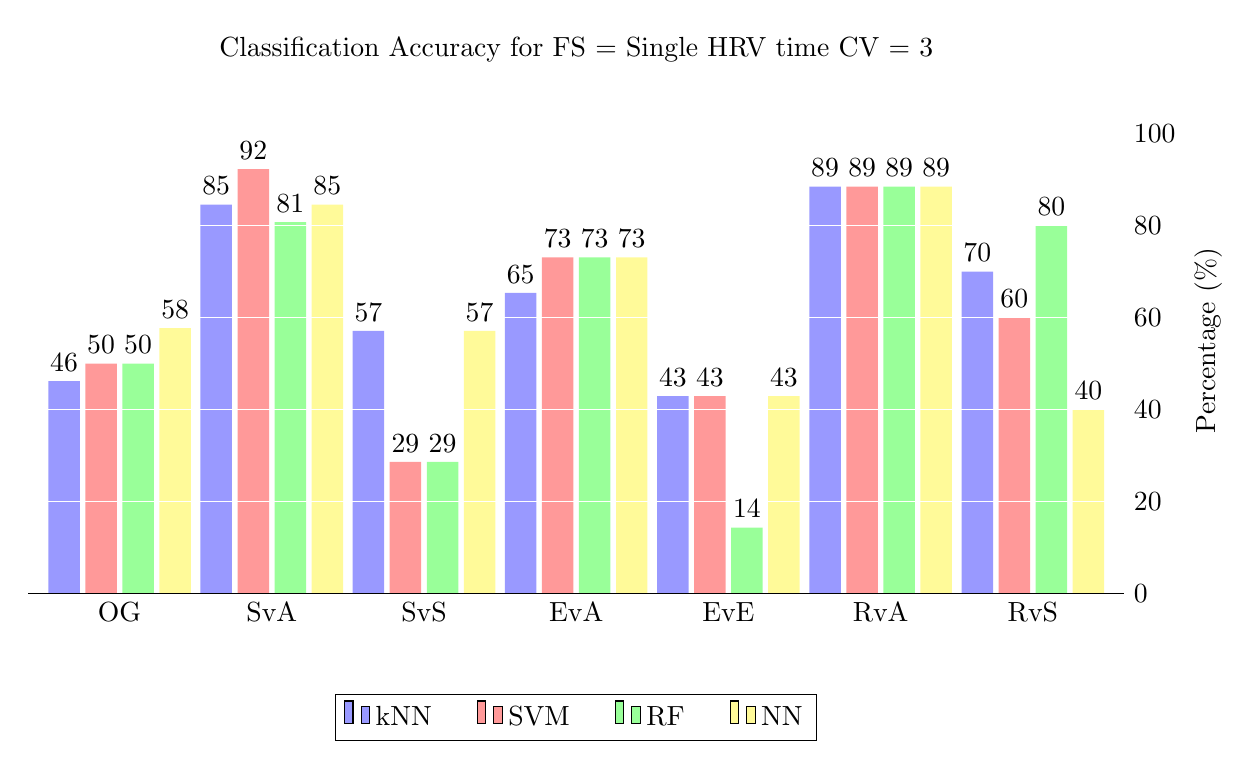
\begin{tikzpicture}
  \centering
  \begin{axis}[
        ybar, axis on top,
        title={Classification Accuracy for FS = Single HRV time CV = 3},
        height=8cm, width=15.5cm,
        bar width=0.4cm,
        ymajorgrids, tick align=inside,
        major grid style={draw=white},
        enlarge y limits={value=.1,upper},
        ymin=0, ymax=100,
        axis x line*=bottom,
        axis y line*=right,
        y axis line style={opacity=0},
        tickwidth=0pt,
        enlarge x limits=true,
        legend style={
            at={(0.5,-0.2)},
            anchor=north,
            legend columns=-1,
            /tikz/every even column/.append style={column sep=0.5cm}
        },
        ylabel={Percentage (\%)},
        symbolic x coords={
           OG, 
           SvA, 
           SvS, 
           EvA, 
           EvE, 
           RvA, 
           RvS},
       xtick=data,
       nodes near coords={
        \pgfmathprintnumber[precision=0]{\pgfplotspointmeta}
       }
    ]
    % kNN
    \addplot [draw=none, fill=blue!40] coordinates {
      (OG, 46.2)
      (SvA, 84.6) 
      (SvS, 57.1)
      (EvA, 65.4) 
      (EvE, 42.9) 
      (RvA, 88.5)
      (RvS, 70.0) };
   % SVM
   \addplot [draw=none,fill=red!40] coordinates {
      (OG, 50)
      (SvA, 92.3) 
      (SvS, 28.6)
      (EvA, 73.1) 
      (EvE, 42.9) 
      (RvA, 88.5)
      (RvS, 60.0) };
   % RF
   \addplot [draw=none, fill=green!40] coordinates {
      (OG, 50.0)
      (SvA, 80.8) 
      (SvS, 28.6)
      (EvA, 73.1) 
      (EvE, 14.3) 
      (RvA, 88.5)
      (RvS, 80.0) };
   % NN
   \addplot [draw=none, fill=yellow!40] coordinates {
      (OG, 57.7)
      (SvA, 84.6) 
      (SvS, 57.1)
      (EvA, 73.1) 
      (EvE, 42.9) 
      (RvA, 88.5)
      (RvS, 40.0) };

    \legend{kNN,SVM,RF,NN}
  \end{axis}
\end{tikzpicture}

% single (hrv t) feature set CV 5
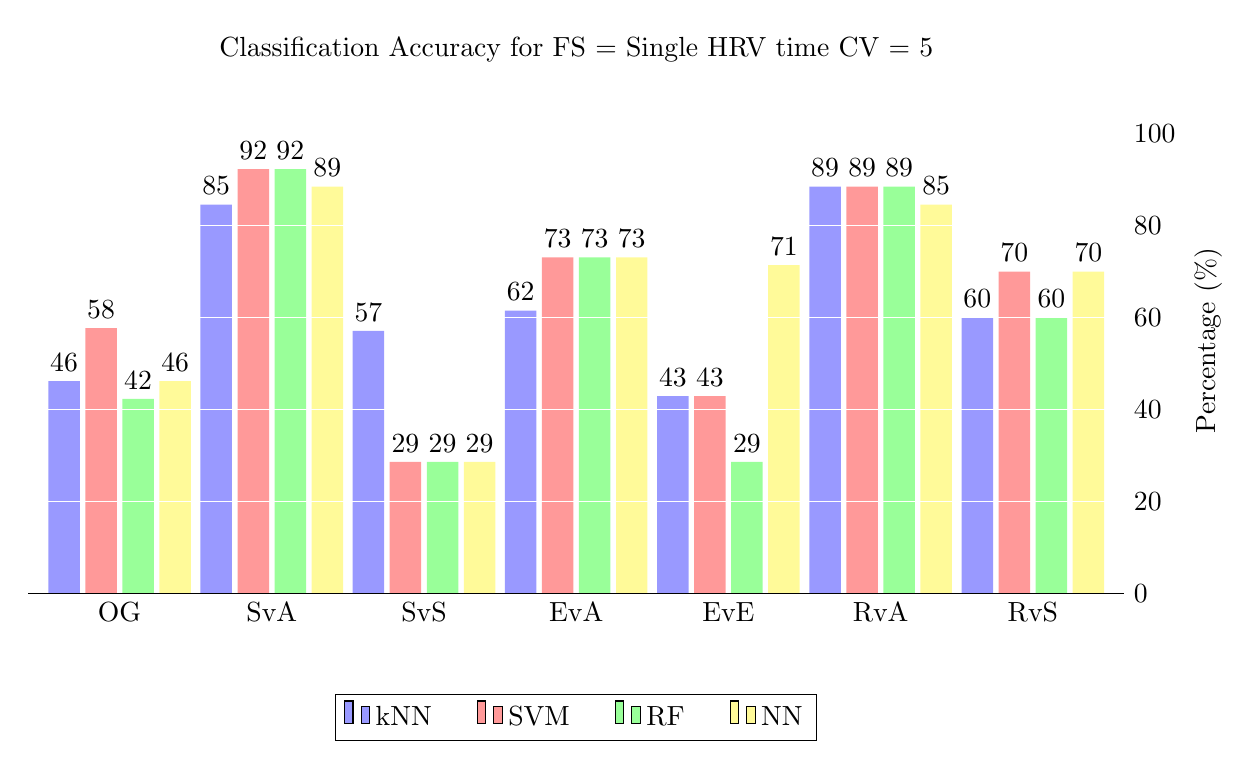
\begin{tikzpicture}
  \centering
  \begin{axis}[
        ybar, axis on top,
        title={Classification Accuracy for FS = Single HRV time CV = 5},
        height=8cm, width=15.5cm,
        bar width=0.4cm,
        ymajorgrids, tick align=inside,
        major grid style={draw=white},
        enlarge y limits={value=.1,upper},
        ymin=0, ymax=100,
        axis x line*=bottom,
        axis y line*=right,
        y axis line style={opacity=0},
        tickwidth=0pt,
        enlarge x limits=true,
        legend style={
            at={(0.5,-0.2)},
            anchor=north,
            legend columns=-1,
            /tikz/every even column/.append style={column sep=0.5cm}
        },
        ylabel={Percentage (\%)},
        symbolic x coords={
           OG, 
           SvA, 
           SvS, 
           EvA, 
           EvE, 
           RvA, 
           RvS},
       xtick=data,
       nodes near coords={
        \pgfmathprintnumber[precision=0]{\pgfplotspointmeta}
       }
    ]
    % kNN
    \addplot [draw=none, fill=blue!40] coordinates {
      (OG, 46.2)
      (SvA, 84.6) 
      (SvS, 57.1)
      (EvA, 61.5) 
      (EvE, 42.9) 
      (RvA, 88.5)
      (RvS, 60.0) };
   % SVM
   \addplot [draw=none,fill=red!40] coordinates {
      (OG, 57.7)
      (SvA, 92.3) 
      (SvS, 28.6)
      (EvA, 73.1) 
      (EvE, 42.9) 
      (RvA, 88.5)
      (RvS, 70.0) };
   % RF
   \addplot [draw=none, fill=green!40] coordinates {
      (OG, 42.3)
      (SvA, 92.3) 
      (SvS, 28.6)
      (EvA, 73.1) 
      (EvE, 28.6) 
      (RvA, 88.5)
      (RvS, 60.0) };
   % NN
   \addplot [draw=none, fill=yellow!40] coordinates {
      (OG, 46.2)
      (SvA, 88.5) 
      (SvS, 28.6)
      (EvA, 73.1) 
      (EvE, 71.4) 
      (RvA, 84.6)
      (RvS, 70.0) };

    \legend{kNN,SVM,RF,NN}
  \end{axis}
\end{tikzpicture}

% single (hrv f) feature set CV 3
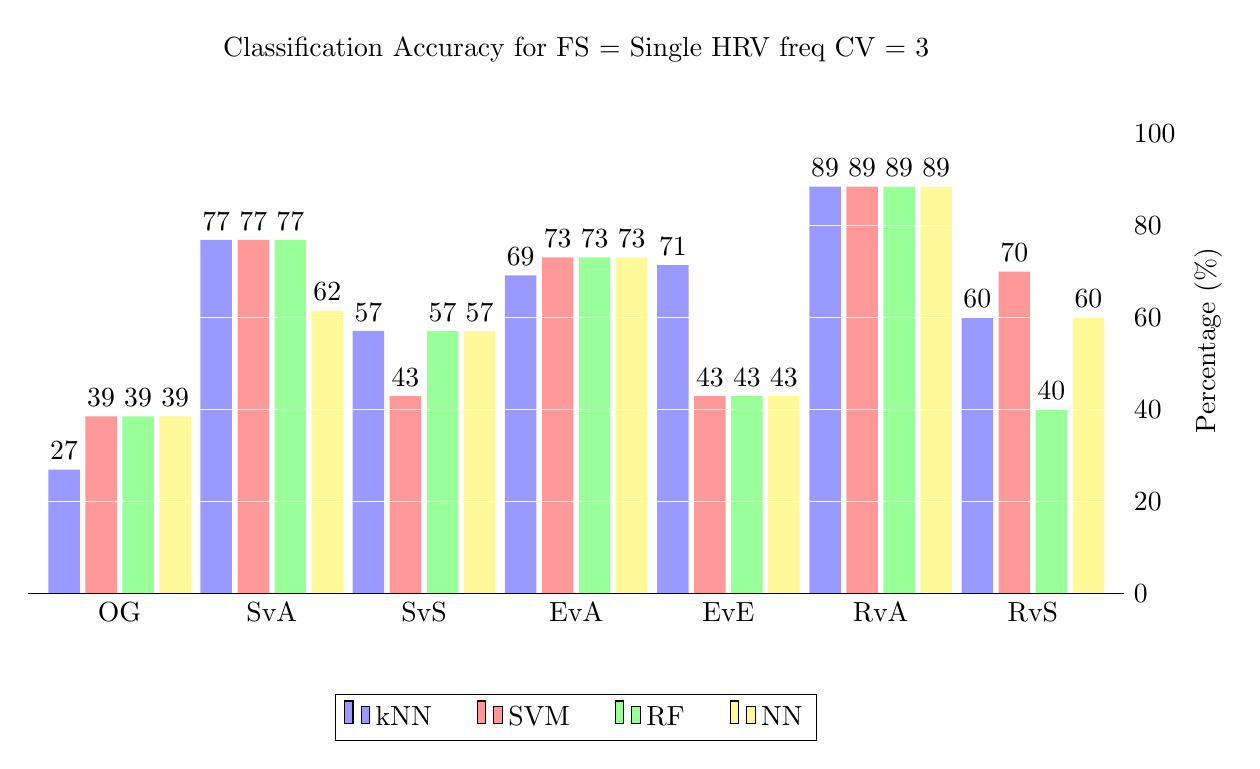
\begin{tikzpicture}
  \centering
  \begin{axis}[
        ybar, axis on top,
        title={Classification Accuracy for FS = Single HRV freq CV = 3},
        height=8cm, width=15.5cm,
        bar width=0.4cm,
        ymajorgrids, tick align=inside,
        major grid style={draw=white},
        enlarge y limits={value=.1,upper},
        ymin=0, ymax=100,
        axis x line*=bottom,
        axis y line*=right,
        y axis line style={opacity=0},
        tickwidth=0pt,
        enlarge x limits=true,
        legend style={
            at={(0.5,-0.2)},
            anchor=north,
            legend columns=-1,
            /tikz/every even column/.append style={column sep=0.5cm}
        },
        ylabel={Percentage (\%)},
        symbolic x coords={
           OG, 
           SvA, 
           SvS, 
           EvA, 
           EvE, 
           RvA, 
           RvS},
       xtick=data,
       nodes near coords={
        \pgfmathprintnumber[precision=0]{\pgfplotspointmeta}
       }
    ]
    % kNN
    \addplot [draw=none, fill=blue!40] coordinates {
      (OG, 26.9)
      (SvA, 76.9) 
      (SvS, 57.1)
      (EvA, 69.2) 
      (EvE, 71.4) 
      (RvA, 88.5)
      (RvS, 60.0) };
   % SVM
   \addplot [draw=none,fill=red!40] coordinates {
      (OG, 38.5)
      (SvA, 76.9) 
      (SvS, 42.9)
      (EvA, 73.1) 
      (EvE, 42.9) 
      (RvA, 88.5)
      (RvS, 70.0) };
   % RF
   \addplot [draw=none, fill=green!40] coordinates {
      (OG, 38.5)
      (SvA, 76.9) 
      (SvS, 57.1)
      (EvA, 73.1) 
      (EvE, 42.9) 
      (RvA, 88.5)
      (RvS, 40.0) };
   % NN
   \addplot [draw=none, fill=yellow!40] coordinates {
      (OG, 38.5)
      (SvA, 61.5) 
      (SvS, 57.1)
      (EvA, 73.1) 
      (EvE, 42.9) 
      (RvA, 88.5)
      (RvS, 60.0) };

    \legend{kNN,SVM,RF,NN}
  \end{axis}
\end{tikzpicture}

% single (hrv f) feature set CV 5
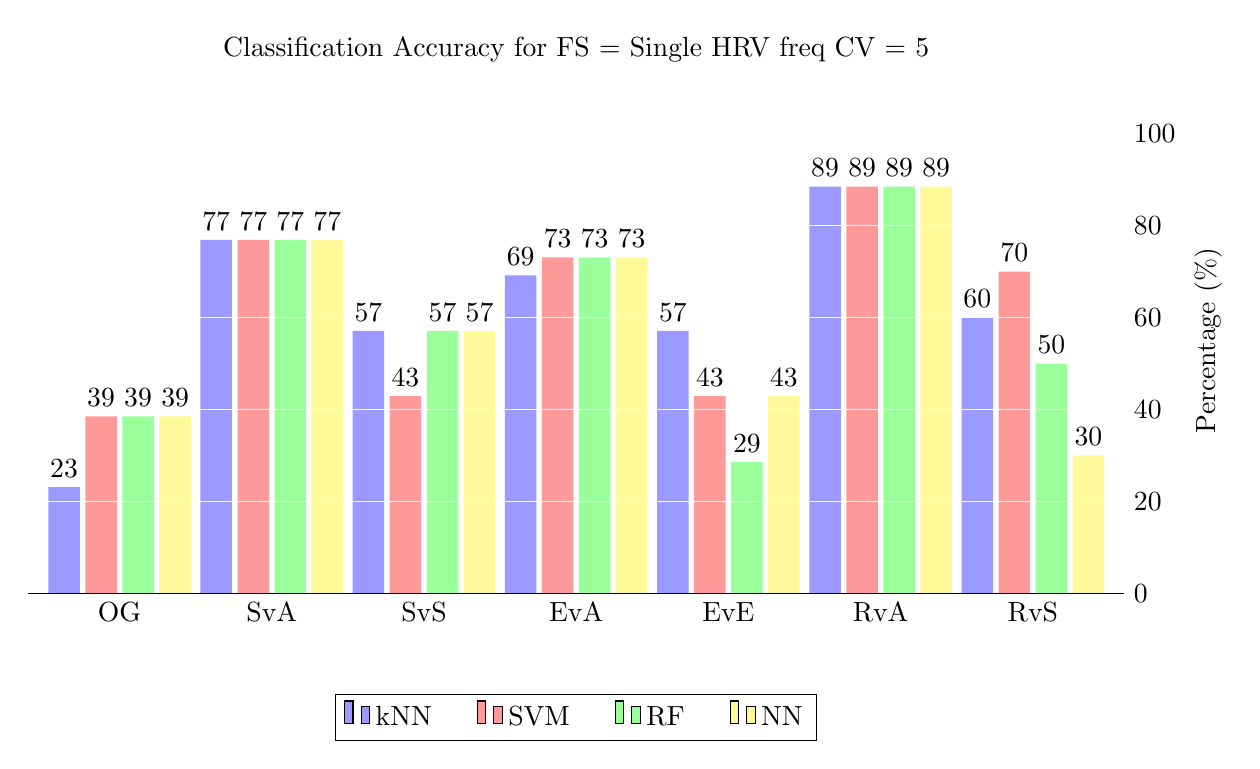
\begin{tikzpicture}
  \centering
  \begin{axis}[
        ybar, axis on top,
        title={Classification Accuracy for FS = Single HRV freq CV = 5},
        height=8cm, width=15.5cm,
        bar width=0.4cm,
        ymajorgrids, tick align=inside,
        major grid style={draw=white},
        enlarge y limits={value=.1,upper},
        ymin=0, ymax=100,
        axis x line*=bottom,
        axis y line*=right,
        y axis line style={opacity=0},
        tickwidth=0pt,
        enlarge x limits=true,
        legend style={
            at={(0.5,-0.2)},
            anchor=north,
            legend columns=-1,
            /tikz/every even column/.append style={column sep=0.5cm}
        },
        ylabel={Percentage (\%)},
        symbolic x coords={
           OG, 
           SvA, 
           SvS, 
           EvA, 
           EvE, 
           RvA, 
           RvS},
       xtick=data,
       nodes near coords={
        \pgfmathprintnumber[precision=0]{\pgfplotspointmeta}
       }
    ]
    % kNN
    \addplot [draw=none, fill=blue!40] coordinates {
      (OG, 23.1)
      (SvA, 76.9) 
      (SvS, 57.1)
      (EvA, 69.2) 
      (EvE, 57.1) 
      (RvA, 88.5)
      (RvS, 60.0) };
   % SVM
   \addplot [draw=none,fill=red!40] coordinates {
      (OG, 38.5)
      (SvA, 76.9) 
      (SvS, 42.9)
      (EvA, 73.1) 
      (EvE, 42.9) 
      (RvA, 88.5)
      (RvS, 70.0) };
   % RF
   \addplot [draw=none, fill=green!40] coordinates {
      (OG, 38.5)
      (SvA, 76.9) 
      (SvS, 57.1)
      (EvA, 73.1) 
      (EvE, 28.6) 
      (RvA, 88.5)
      (RvS, 50.0) };
   % NN
   \addplot [draw=none, fill=yellow!40] coordinates {
      (OG, 38.5)
      (SvA, 76.9) 
      (SvS, 57.1)
      (EvA, 73.1) 
      (EvE, 42.9) 
      (RvA, 88.5)
      (RvS, 30.0) };

    \legend{kNN,SVM,RF,NN}
  \end{axis}
\end{tikzpicture}

% single (gsr t) feature set CV 3
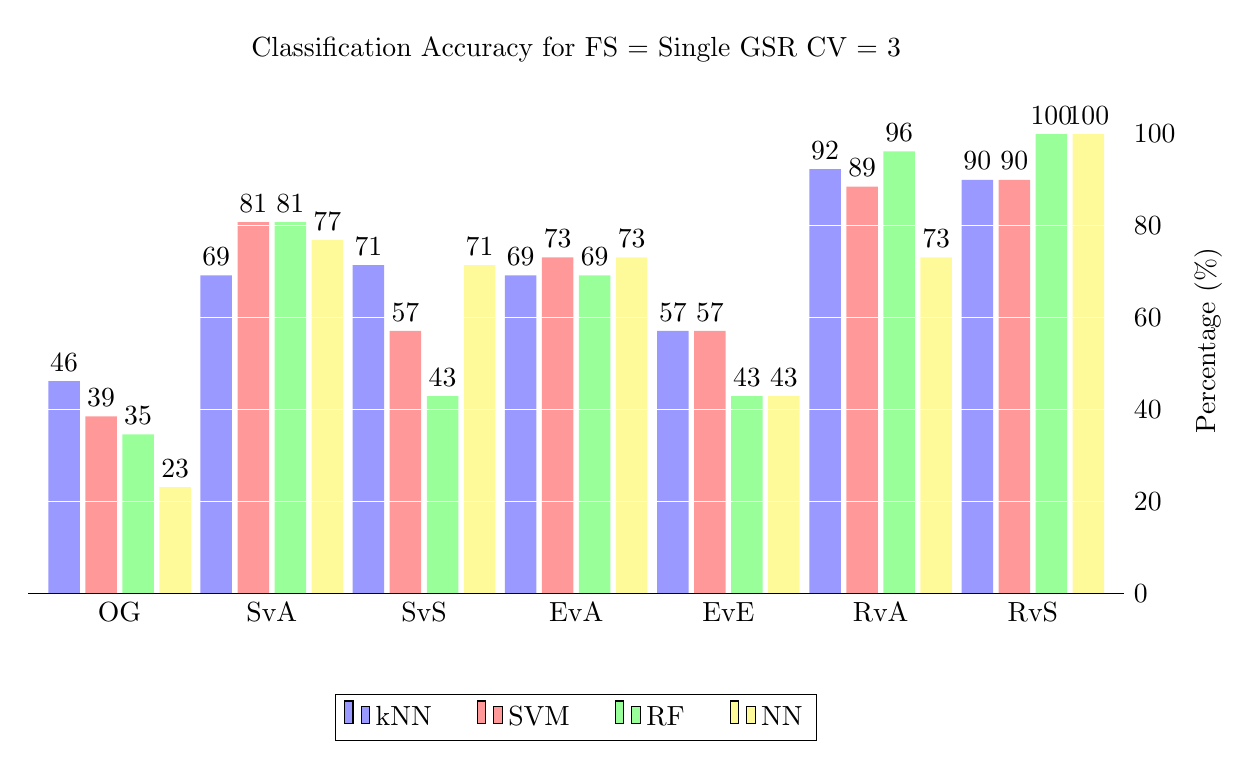
\begin{tikzpicture}
  \centering
  \begin{axis}[
        ybar, axis on top,
        title={Classification Accuracy for FS = Single GSR CV = 3},
        height=8cm, width=15.5cm,
        bar width=0.4cm,
        ymajorgrids, tick align=inside,
        major grid style={draw=white},
        enlarge y limits={value=.1,upper},
        ymin=0, ymax=100,
        axis x line*=bottom,
        axis y line*=right,
        y axis line style={opacity=0},
        tickwidth=0pt,
        enlarge x limits=true,
        legend style={
            at={(0.5,-0.2)},
            anchor=north,
            legend columns=-1,
            /tikz/every even column/.append style={column sep=0.5cm}
        },
        ylabel={Percentage (\%)},
        symbolic x coords={
           OG, 
           SvA, 
           SvS, 
           EvA, 
           EvE, 
           RvA, 
           RvS},
       xtick=data,
       nodes near coords={
        \pgfmathprintnumber[precision=0]{\pgfplotspointmeta}
       }
    ]
    % kNN
    \addplot [draw=none, fill=blue!40] coordinates {
      (OG, 46.2)
      (SvA, 69.2) 
      (SvS, 71.4)
      (EvA, 69.2) 
      (EvE, 57.1) 
      (RvA, 92.3)
      (RvS, 90.0) };
   % SVM
   \addplot [draw=none,fill=red!40] coordinates {
      (OG, 38.5)
      (SvA, 80.8) 
      (SvS, 57.1)
      (EvA, 73.1) 
      (EvE, 57.1) 
      (RvA, 88.5)
      (RvS, 90.0) };
   % RF
   \addplot [draw=none, fill=green!40] coordinates {
      (OG, 34.6)
      (SvA, 80.8) 
      (SvS, 42.9)
      (EvA, 69.2) 
      (EvE, 42.9) 
      (RvA, 96.2)
      (RvS, 100.0) };
   % NN
   \addplot [draw=none, fill=yellow!40] coordinates {
      (OG, 23.1)
      (SvA, 76.9) 
      (SvS, 71.4)
      (EvA, 73.1) 
      (EvE, 42.9) 
      (RvA, 73.1)
      (RvS, 100.0) };

    \legend{kNN,SVM,RF,NN}
  \end{axis}
\end{tikzpicture}

% single (gsr t) feature set CV 5
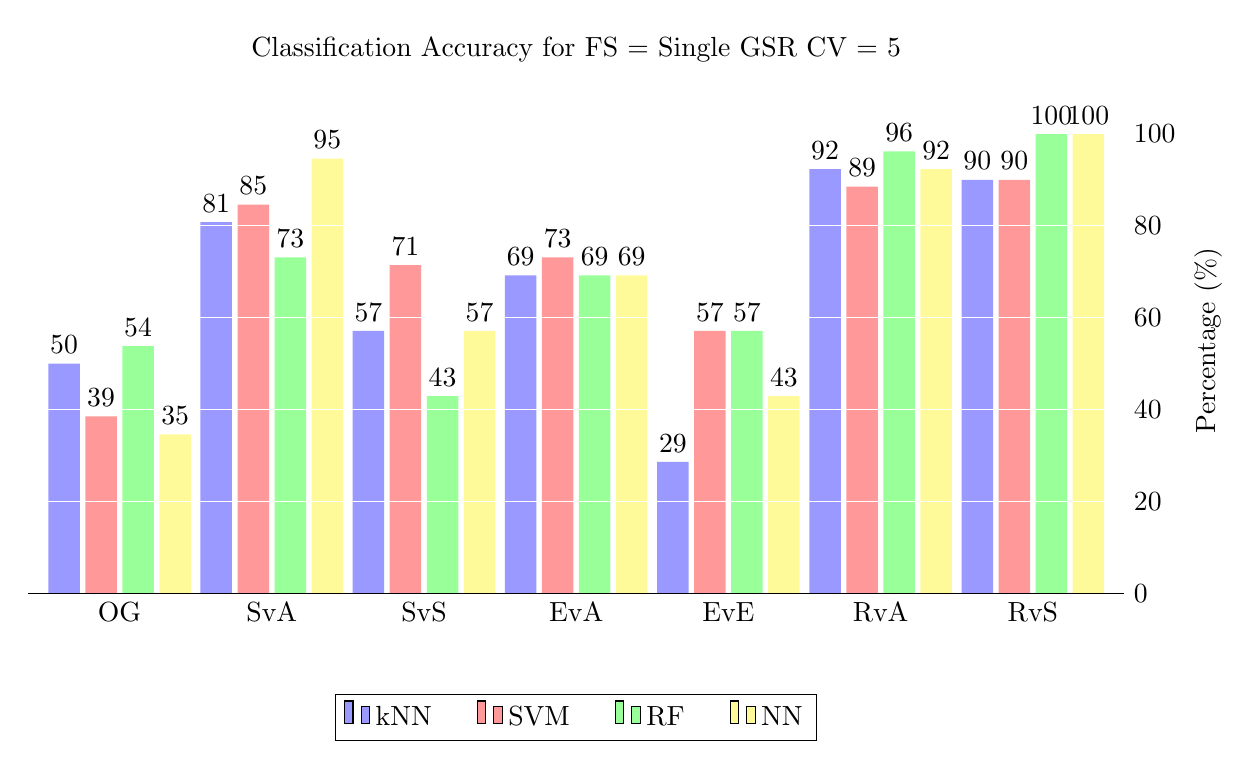
\begin{tikzpicture}
  \centering
  \begin{axis}[
        ybar, axis on top,
        title={Classification Accuracy for FS = Single GSR CV = 5},
        height=8cm, width=15.5cm,
        bar width=0.4cm,
        ymajorgrids, tick align=inside,
        major grid style={draw=white},
        enlarge y limits={value=.1,upper},
        ymin=0, ymax=100,
        axis x line*=bottom,
        axis y line*=right,
        y axis line style={opacity=0},
        tickwidth=0pt,
        enlarge x limits=true,
        legend style={
            at={(0.5,-0.2)},
            anchor=north,
            legend columns=-1,
            /tikz/every even column/.append style={column sep=0.5cm}
        },
        ylabel={Percentage (\%)},
        symbolic x coords={
           OG, 
           SvA, 
           SvS, 
           EvA, 
           EvE, 
           RvA, 
           RvS},
       xtick=data,
       nodes near coords={
        \pgfmathprintnumber[precision=0]{\pgfplotspointmeta}
       }
    ]
    % kNN
    \addplot [draw=none, fill=blue!40] coordinates {
      (OG, 50.0)
      (SvA, 80.8) 
      (SvS, 57.1)
      (EvA, 69.2) 
      (EvE, 28.6) 
      (RvA, 92.3)
      (RvS, 90.0) };
   % SVM
   \addplot [draw=none,fill=red!40] coordinates {
      (OG, 38.5)
      (SvA, 84.6) 
      (SvS, 71.4)
      (EvA, 73.1) 
      (EvE, 57.1) 
      (RvA, 88.5)
      (RvS, 90.0) };
   % RF
   \addplot [draw=none, fill=green!40] coordinates {
      (OG, 53.8)
      (SvA, 73.1) 
      (SvS, 42.9)
      (EvA, 69.2) 
      (EvE, 57.1) 
      (RvA, 96.2)
      (RvS, 100.0) };
   % NN
   \addplot [draw=none, fill=yellow!40] coordinates {
      (OG, 34.6)
      (SvA, 94.6) 
      (SvS, 57.1)
      (EvA, 69.2) 
      (EvE, 42.9) 
      (RvA, 92.3)
      (RvS, 100.0) };

    \legend{kNN,SVM,RF,NN}
  \end{axis}
\end{tikzpicture}

% single (temp t) feature set CV 3
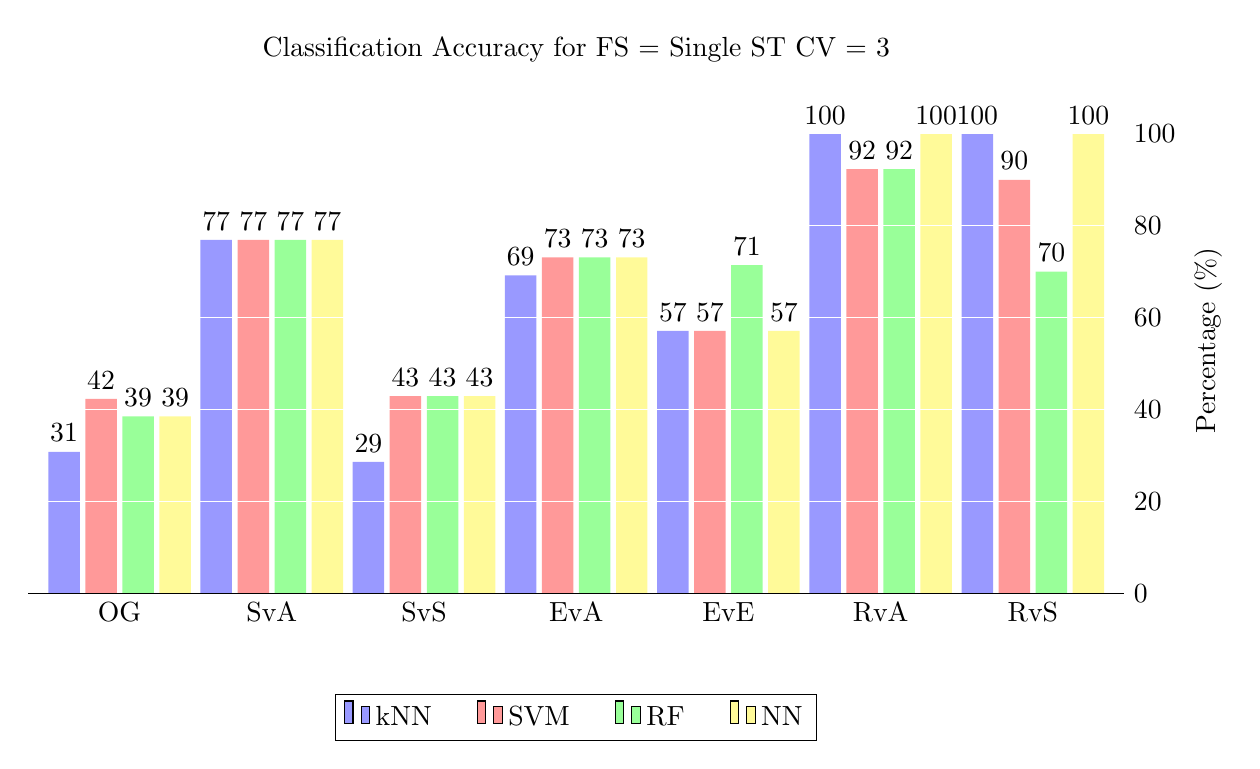
\begin{tikzpicture}
  \centering
  \begin{axis}[
        ybar, axis on top,
        title={Classification Accuracy for FS = Single ST CV = 3},
        height=8cm, width=15.5cm,
        bar width=0.4cm,
        ymajorgrids, tick align=inside,
        major grid style={draw=white},
        enlarge y limits={value=.1,upper},
        ymin=0, ymax=100,
        axis x line*=bottom,
        axis y line*=right,
        y axis line style={opacity=0},
        tickwidth=0pt,
        enlarge x limits=true,
        legend style={
            at={(0.5,-0.2)},
            anchor=north,
            legend columns=-1,
            /tikz/every even column/.append style={column sep=0.5cm}
        },
        ylabel={Percentage (\%)},
        symbolic x coords={
           OG, 
           SvA, 
           SvS, 
           EvA, 
           EvE, 
           RvA, 
           RvS},
       xtick=data,
       nodes near coords={
        \pgfmathprintnumber[precision=0]{\pgfplotspointmeta}
       }
    ]
    % kNN
    \addplot [draw=none, fill=blue!40] coordinates {
      (OG, 30.8)
      (SvA, 76.9) 
      (SvS, 28.6)
      (EvA, 69.2) 
      (EvE, 57.1) 
      (RvA, 100.0)
      (RvS, 100.0) };
   % SVM
   \addplot [draw=none,fill=red!40] coordinates {
      (OG, 42.3)
      (SvA, 76.9) 
      (SvS, 42.9)
      (EvA, 73.1) 
      (EvE, 57.1) 
      (RvA, 92.3)
      (RvS, 90.0) };
   % RF
   \addplot [draw=none, fill=green!40] coordinates {
      (OG, 38.5)
      (SvA, 76.9) 
      (SvS, 42.9)
      (EvA, 73.1) 
      (EvE, 71.4) 
      (RvA, 92.3)
      (RvS, 70.0) };
   % NN
   \addplot [draw=none, fill=yellow!40] coordinates {
      (OG, 38.5)
      (SvA, 76.9) 
      (SvS, 42.9)
      (EvA, 73.1) 
      (EvE, 57.1) 
      (RvA, 100.0)
      (RvS, 100.0) };

    \legend{kNN,SVM,RF,NN}
  \end{axis}
\end{tikzpicture}

% single (temp t) feature set CV 5
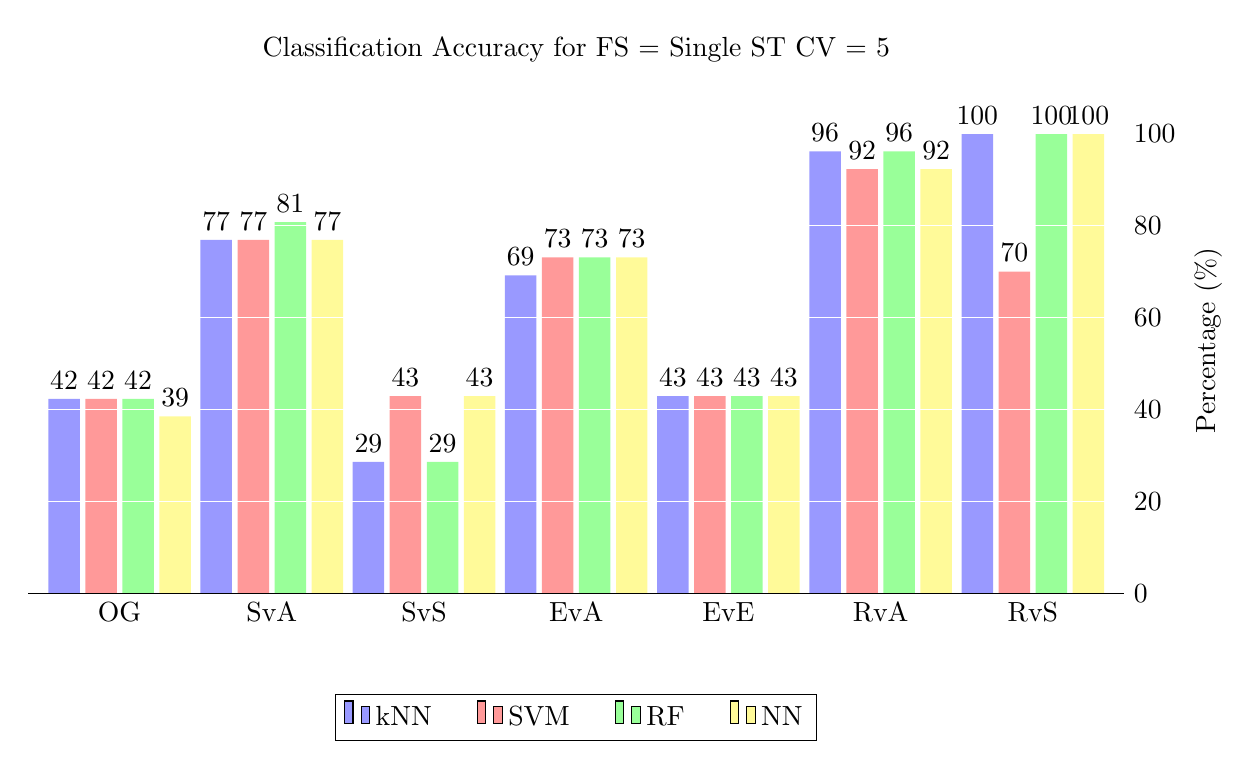
\begin{tikzpicture}
  \centering
  \begin{axis}[
        ybar, axis on top,
        title={Classification Accuracy for FS = Single ST CV = 5},
        height=8cm, width=15.5cm,
        bar width=0.4cm,
        ymajorgrids, tick align=inside,
        major grid style={draw=white},
        enlarge y limits={value=.1,upper},
        ymin=0, ymax=100,
        axis x line*=bottom,
        axis y line*=right,
        y axis line style={opacity=0},
        tickwidth=0pt,
        enlarge x limits=true,
        legend style={
            at={(0.5,-0.2)},
            anchor=north,
            legend columns=-1,
            /tikz/every even column/.append style={column sep=0.5cm}
        },
        ylabel={Percentage (\%)},
        symbolic x coords={
           OG, 
           SvA, 
           SvS, 
           EvA, 
           EvE, 
           RvA, 
           RvS},
       xtick=data,
       nodes near coords={
        \pgfmathprintnumber[precision=0]{\pgfplotspointmeta}
       }
    ]
    % kNN
    \addplot [draw=none, fill=blue!40] coordinates {
      (OG, 42.3)
      (SvA, 76.9) 
      (SvS, 28.6)
      (EvA, 69.2) 
      (EvE, 42.9) 
      (RvA, 96.2)
      (RvS, 100.0) };
   % SVM
   \addplot [draw=none,fill=red!40] coordinates {
      (OG, 42.3)
      (SvA, 76.9) 
      (SvS, 42.9)
      (EvA, 73.1) 
      (EvE, 42.9) 
      (RvA, 92.3)
      (RvS, 70.0) };
   % RF
   \addplot [draw=none, fill=green!40] coordinates {
      (OG, 42.3)
      (SvA, 80.8) 
      (SvS, 28.6)
      (EvA, 73.1) 
      (EvE, 42.9) 
      (RvA, 96.2)
      (RvS, 100.0) };
   % NN
   \addplot [draw=none, fill=yellow!40] coordinates {
      (OG, 38.5)
      (SvA, 76.9) 
      (SvS, 42.9)
      (EvA, 73.1) 
      (EvE, 42.9) 
      (RvA, 92.3)
      (RvS, 100.0) };

    \legend{kNN,SVM,RF,NN}
  \end{axis}
\end{tikzpicture}

However, in this form the results have rather low significance, as the sheer amount of plots hinders proper evaluation. Therefore, we constructed the following tables to improve data illustration. We listed the average accuracy for each classifier based on either feature selection (see \ref{perffb}) or data set (see \ref{perfdb}) to providing insight on their respective effects on individual algorithm performances. \\
% Average algorithm performance over all data sets for a single feature
\begin{table}
\caption[Algorithm Performance: Feature Based]{Feature Based Performance}
\begin{center}
\begin{tabular}{cccc}
\hline 
\thead{\makecell[c]{Algorithm}} & \thead{\makecell[c]{Accuracy (\%)}} & \thead{\makecell[c]{Algorithm}} & \thead{\makecell[c]{Accuracy (\%)}}\\ 
\multicolumn{2}{c}{Original} & \multicolumn{2}{c}{Single HRV Freq.} \\ 
 & & &\\
\hline
 & & &\\
kNN & 63 & kNN & 63\\ 
SVM & 68 & SVM & 62\\
RT & 68 & RT & 59\\
NN & 69 & NN & 59\\
 & & &\\
\multicolumn{2}{c}{Reduced T} & \multicolumn{2}{c}{Single GSR} \\
 & & &\\
\hline
 & & &\\
kNN & 64 & kNN & 69\\
SVM & 73 & SVM & 71\\
RT & 69 & RT & 69\\
NN & 71 & NN & 68\\
 & & &\\
\multicolumn{2}{c}{Reduced F} & \multicolumn{2}{c}{Single ST} \\ 
 & & & \\
\hline
 & & & \\
kNN & 63 & kNN & 66\\
SVM & 63 & SVM & 65\\
RT & 66 & RT & 66\\
NN & 60 & NN & 68\\
 & & & \\
\multicolumn{2}{c}{Single HRV Time} & \multicolumn{2}{c}{Averages}\\
 & & &\\
\hline
 & & & \\
kNN & 64 & kNN & 65\\
SVM & 64 & SVM & 67\\
RT & 59 & RT & 65\\
NN & 65 & NN & 66\\
 & & & \\
\hline
\end{tabular} \label{perffb}
\end{center}
\end{table}

% Average algorithm performance over all features sets for individual data sets
\begin{table}
\caption[Algorithm Performance: Data Based]{Data Based Performance}
\begin{center}
\begin{tabular}{cccc}
\hline 
\thead{\makecell[c]{Algorithm}} & \thead{\makecell[c]{Accuracy (\%)}} & \thead{\makecell[c]{Algorithm}} & \thead{\makecell[c]{Accuracy (\%)}}\\ 
\multicolumn{2}{c}{Original} & \multicolumn{2}{c}{SvA} \\ 
 & & &\\
\hline
 & & &\\
kNN & 36 & kNN & 79\\ 
SVM & 46 & SVM & 85\\
RT & 42 & RT & 81\\
NN & 41 & NN & 85\\
 & & &\\
\multicolumn{2}{c}{SvS} & \multicolumn{2}{c}{EvA} \\
 & & &\\
\hline
 & & &\\
kNN & 54 & kNN & 68 \\ 
SVM & 46 & SVM & 73 \\
RT & 45 & RT & 72 \\
NN & 49 & NN & 72 \\
 & & &\\
\multicolumn{2}{c}{EvE} & \multicolumn{2}{c}{RvA} \\ 
 & & & \\
\hline
 & & & \\
kNN & 53 & kNN & 91\\ 
SVM & 48 & SVM & 90\\
RT & 41 & RT & 92\\
NN & 47 & NN & 90\\
 & & & \\
\multicolumn{2}{c}{RvS} & \multicolumn{2}{c}{Averages}\\
 & & &\\
\hline
 & & & \\
kNN & 71 & kNN & 65\\ 
SVM & 78 & SVM & 67\\
RT & 81 & RT & 65\\
NN & 77 & NN & 66\\
 & & & \\
\hline
\end{tabular} \label{perfdb}
\end{center}
\end{table}

\newpage
Lastly, we calculated classification accuracies for individual data sets (see \ref{aadb}), as well as individual feature sets (see \ref{aafb}) using the collective performance average of all four algorithms.\\
% average performance of all classifier based on feature set
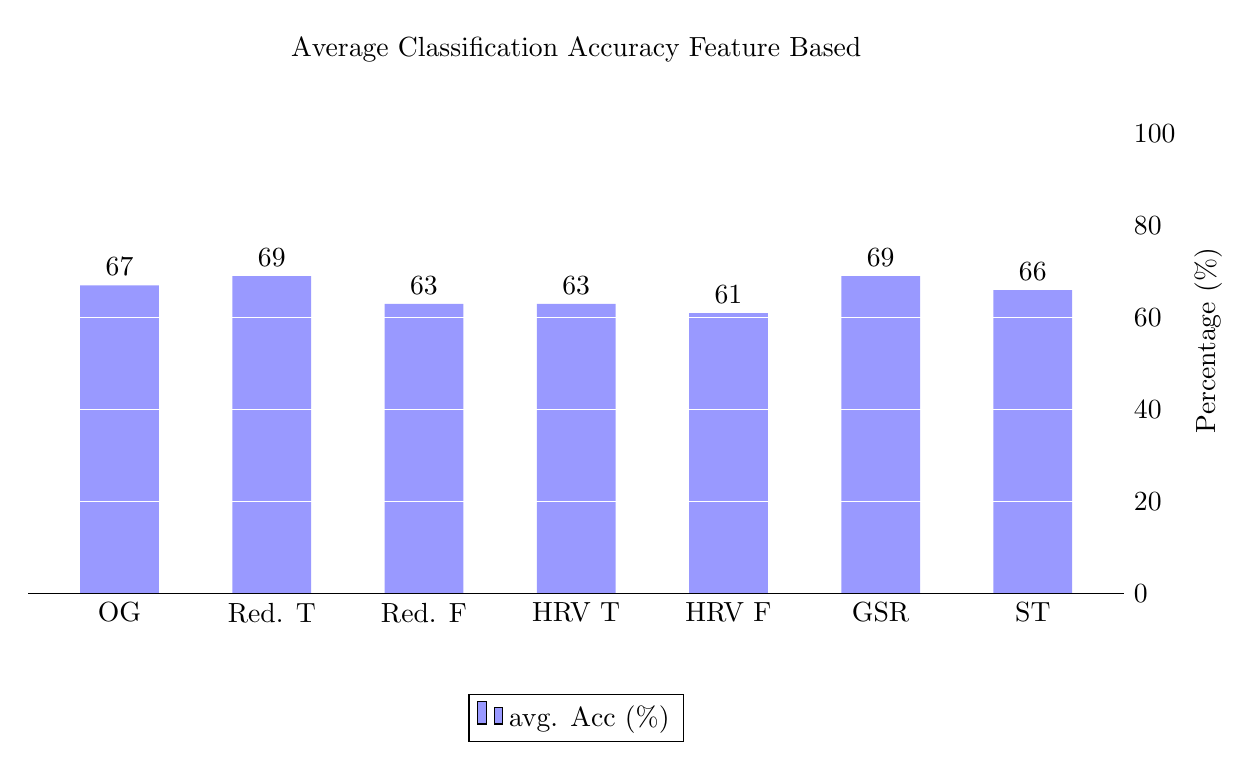
\begin{tikzpicture}
  \centering
  \begin{axis}[
        ybar, axis on top,
        title={Average Classification Accuracy Feature Based},
        height=8cm, width=15.5cm,
        bar width=1.0cm,
        ymajorgrids, tick align=inside,
        major grid style={draw=white},
        enlarge y limits={value=.1,upper},
        ymin=0, ymax=100,
        axis x line*=bottom,
        axis y line*=right,
        y axis line style={opacity=0},
        tickwidth=0pt,
        enlarge x limits=true,
        legend style={
            at={(0.5,-0.2)},
            anchor=north,
            legend columns=-1,
            /tikz/every even column/.append style={column sep=0.5cm}
        },
        ylabel={Percentage (\%)},
        symbolic x coords={
           OG, 
           Red. T, 
           Red. F, 
           HRV T, 
           HRV F, 
           GSR, 
           ST},
       xtick=data,
       nodes near coords={
        \pgfmathprintnumber[precision=0]{\pgfplotspointmeta}
       }
    ]
    
    \addplot [draw=none, fill=blue!40] coordinates {
      (OG, 67)
      (Red. T, 69) 
      (Red. F, 63)
      (HRV T, 63) 
      (HRV F, 61) 
      (GSR, 69)
      (ST, 66) };
    \legend{avg. Acc (\%)}
  \end{axis}
\end{tikzpicture}\label{aafb}

% Average Classification Accuracy Data Based
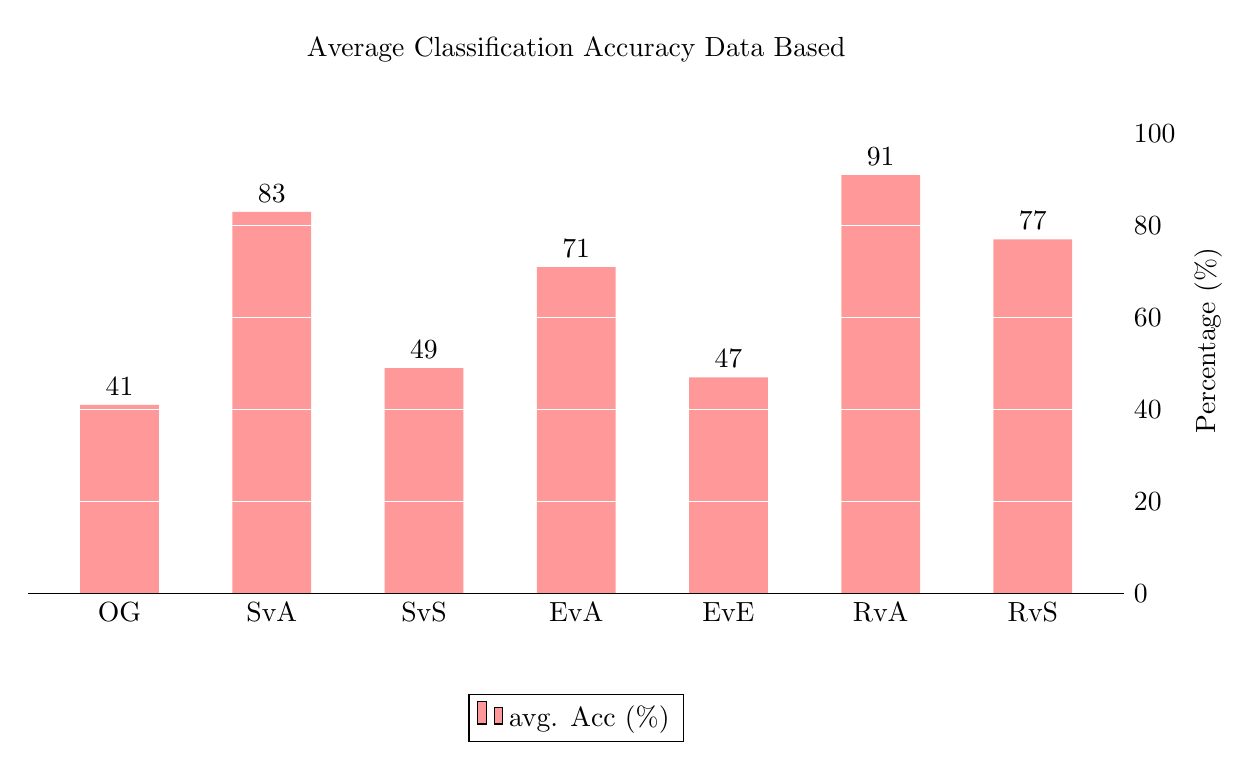
\begin{tikzpicture}
  \centering
  \begin{axis}[
        ybar, axis on top,
        title={Average Classification Accuracy Data Based},
        height=8cm, width=15.5cm,
        bar width=1.0cm,
        ymajorgrids, tick align=inside,
        major grid style={draw=white},
        enlarge y limits={value=.1,upper},
        ymin=0, ymax=100,
        axis x line*=bottom,
        axis y line*=right,
        y axis line style={opacity=0},
        tickwidth=0pt,
        enlarge x limits=true,
        legend style={
            at={(0.5,-0.2)},
            anchor=north,
            legend columns=-1,
            /tikz/every even column/.append style={column sep=0.5cm}
        },
        ylabel={Percentage (\%)},
        symbolic x coords={
           OG, 
           SvA, 
           SvS, 
           EvA, 
           EvE, 
           RvA, 
           RvS},
       xtick=data,
       nodes near coords={
        \pgfmathprintnumber[precision=0]{\pgfplotspointmeta}
       }
    ]
    \addplot [draw=none, fill=red!40] coordinates {
      (OG, 41)
      (SvA, 83) 
      (SvS, 49)
      (EvA, 71) 
      (EvE, 47) 
      (RvA, 91)
      (RvS, 77) };
    \legend{avg. Acc (\%)}
  \end{axis}
\end{tikzpicture}\label{aadb}
	
	